Das L"osen von Eigenwertproblemen ist eine Standarddisziplin in der
numerischen linearen Algebra. Die konkrete Problemstellung dabei lautet: Zu gegebenen Matrizen $A,B\in\Cnn$ sollen Paare $(\lambda, x)$ mit $\lambda\in\C$ und $x\in\Co$ gefunden werden, welche
der Gleichung
\begin{equation}\label{chap1:eq:eigenproblem}
Ax = \lambda Bx
\end{equation}

gen"ugen. Solchen \emph{Eigenwertgleichungen} begegnet man in ganz unterschiedlichen Kontexten.
So sind sie beispielsweise bei der Bestimmung von Eigenfrequenzen oder dem Ermitteln von Fixpunkten beim
Rotieren eines Fu"sballs\footnote{Hier wird auf den bekannten
\emph{Satz vom Fu"sball} angespielt. Dieser besagt, dass auf einem Fußball
zwei Punkte existieren, die zu Spielbeginn und zur Halbzeit
an der gleichen Stelle liegen -- informell formuliert.} ebenso wie beim
Untersuchen des PageRanks\footnote{
Siehe Abschnitt zwei in ~\cite{page}.
} einer Website von
Bedeutung. Entsprechend strotz der Kanon von angebotenen numerischen
L"osungsmethoden von Vielfalt und Virtuosit"at.\footnote{Dies best"atigt sich beispielsweise bei einem Blick in das Inhaltsverzeichnis von ~\cite{stewart}.}\\

Nun mag der Fall eintreten, da es notwendig wird, lediglich eine Teilmenge
aus der Menge aller Eigenpaare zu untersuchen. Betrachten wir zur Illustration folgende Abbildung.

\begin{figure}[h!]
  \centering
  \resizebox{.4\linewidth}{!}{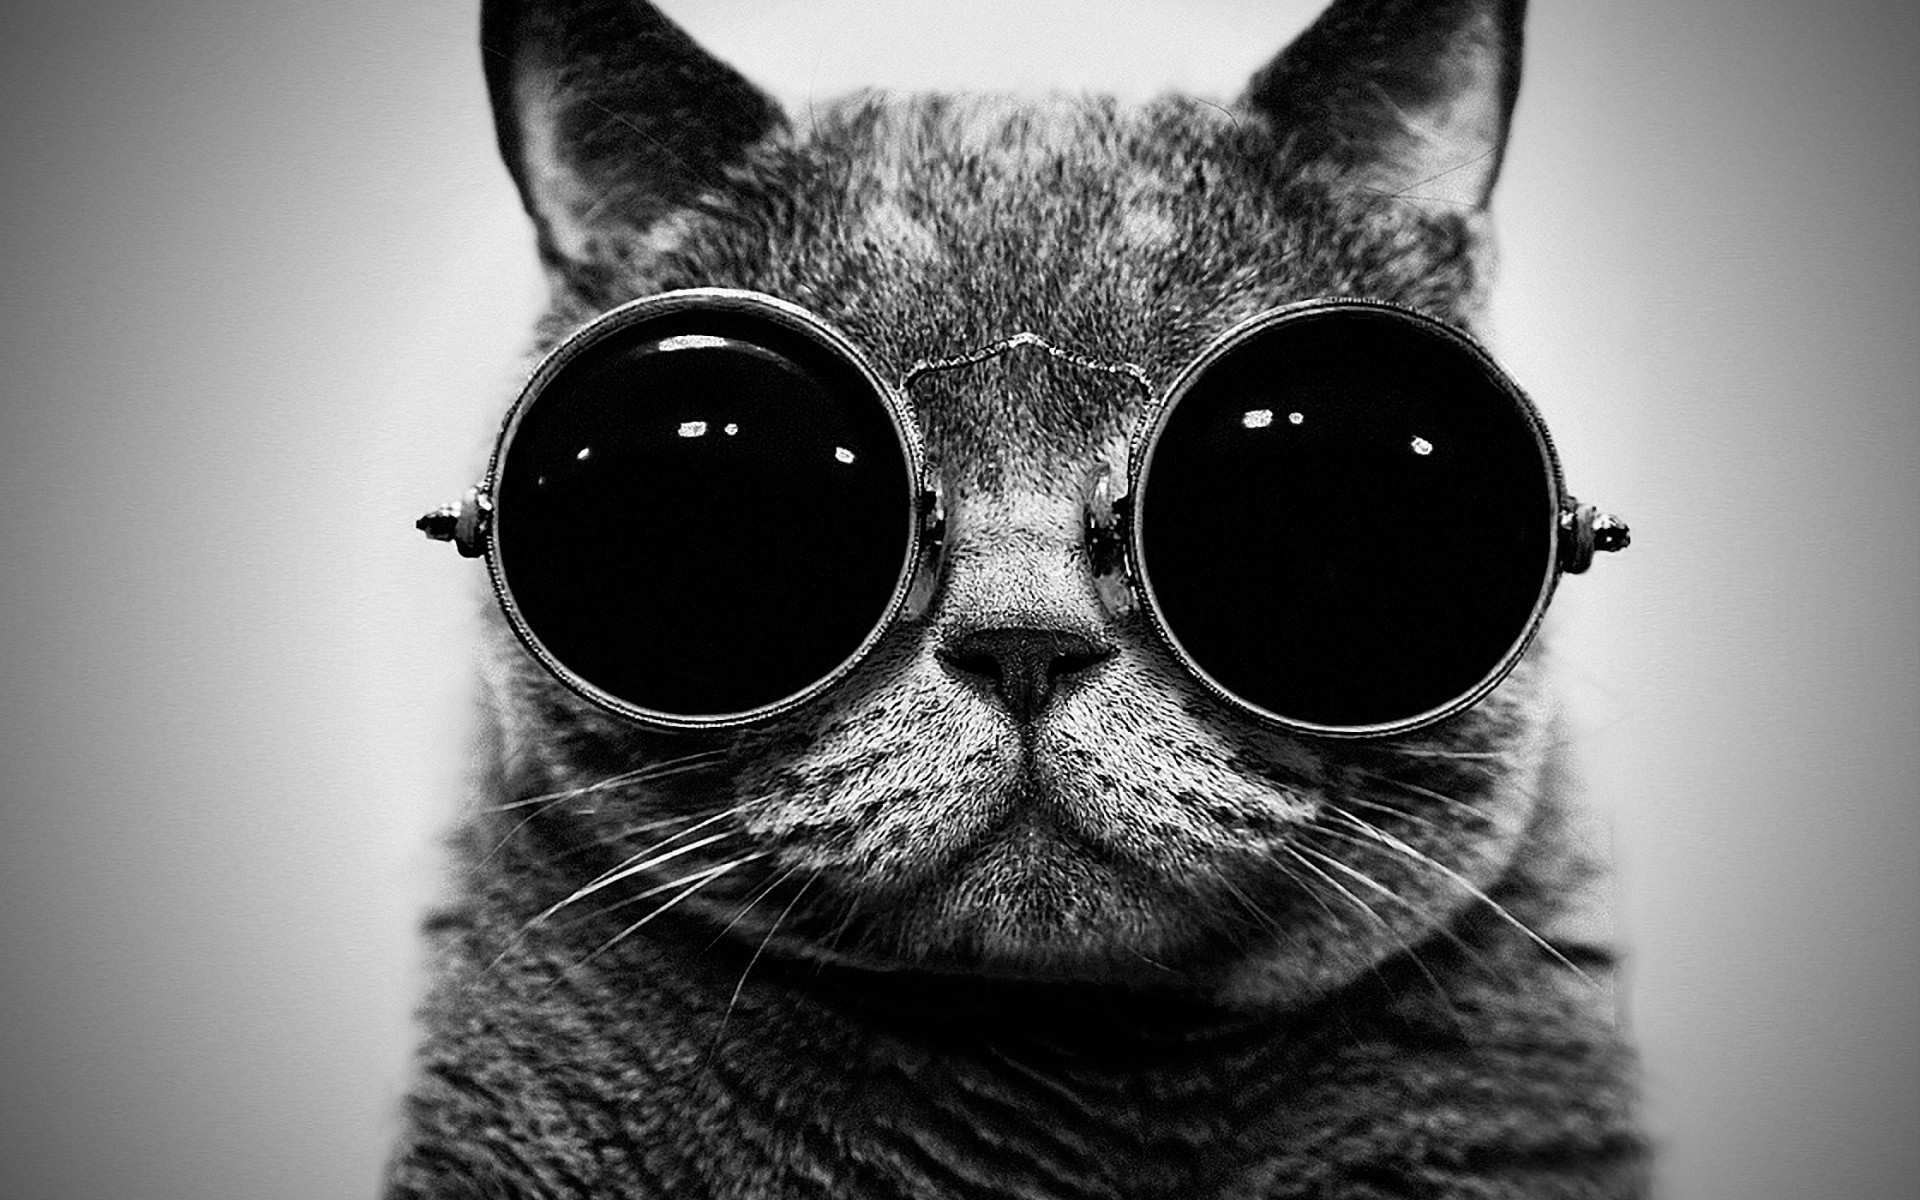
\includegraphics{images/Cat}}
  \caption{\glqq Mind Games of Ozzy\grqq\ von Andy Prokh.}\label{chap1:im:cat}
\end{figure}

%Diese Foto ben"otigt in der Originalgr"o"se einen Speicherplatz von \textcolor{red}{9000mb}.%\footnote{Das Foto aus Abbildung \ref{chap1:im:cat} wurde dabei mit einer \textcolor{red}{tollen Kamera} gemacht.}
Man stelle sich vor, man wolle dieses Bild komprimieren, um den ben"otigten Speicherplatz zu reduzieren.
Dies l"asst sich beispielsweise mit einer sogenannten \emph{Singul"arwertzerlegung} -- von Numerikern liebevoll als das \emph{Schweizer Taschenmesser der linearen Algebra} bezeichnet -- bewerkstelligen.\\

Da es sich bei Abbildung \ref{chap1:im:cat} um ein Schwarz-Wei"s-Bild handelt, l"asst sie sich als eine Matrix $M$ auffassen, deren Eintr"age die Grauwerte der einzelnen Pixel repr"asentieren.
Unter Anwendung des Satzes von der Singul"arwertzerlegung\footnote{Eine Formulierung ohne Beweis ist mit Satz \ref{app:thm:svd} -- zu finden im Anhang -- gegeben.} l"asst sich nun das Bild der Katze durch eine Folge von Matrizen niedrigeren Ranges approximieren.
Man berechnet hierf"ur die Wurzeln der von Null verschiedenen Eigenwerte von $M^H M$ und verwendet dann diese sogenannten \emph{Singul"arwerte} um die Matrix $M$ zu rekonstruieren.
Auf weitere Details "uber den hinter diesem Verfahren stehenden Algorithmus wollen wir an dieser Stelle verzichten.\\

Die Matrix $M$ hat in unserem Beispiel mehr als 700 Singul"arwerte. Die Frage ist nun, ob wir uns von einigen Singul"arwerten trennen k"onnen und dennoch eine akzeptable Bildqualit"at aufrecht erhalten k"onnen.
Insbesondere ist wichtig zu wissen, welche dieser Werte entscheidend f"ur die Rekonstruktion sind.\\

Dazu nehmen wir uns die $n\in\N$ Singul"arwerte $\sigma_1,\ldots,\sigma_n$ her. Ohne Einschr"ankung seien diese so nummeriert, dass $\sigma_1 \ge \ldots \ge \sigma_n$ gilt. Sollte dies nicht der Fall sein, nummerieren wir einfach um.
Nun filtern wir nach eigenen Kriterien Teilmengen aus den Singul"arwerten, beziehungsweise den Eigenwerten von $M^H M$ heraus und rekonstruieren mit deren Hilfe die Abbildung \ref{chap1:im:cat}.\\

Es sei an dieser Stelle darauf hingewiesen, dass die folgendenen Beurteilungen der Bildqualit"at nicht mathematisch begr"undet sind.
Die Eindr"ucke entstammen dem pers"onlichen Empfinden des Autors, sowie den Aussagen einer kleinen Testgruppe von Studierenden des Fachs Mathematik.\\

Beginnen wir mit einer mehr oder weniger willk"urlichen Auswahl von Singul"arwerten (SW).

\begin{figure}[h!]
\center
\begin{subfigure}[c]{.3\textwidth}
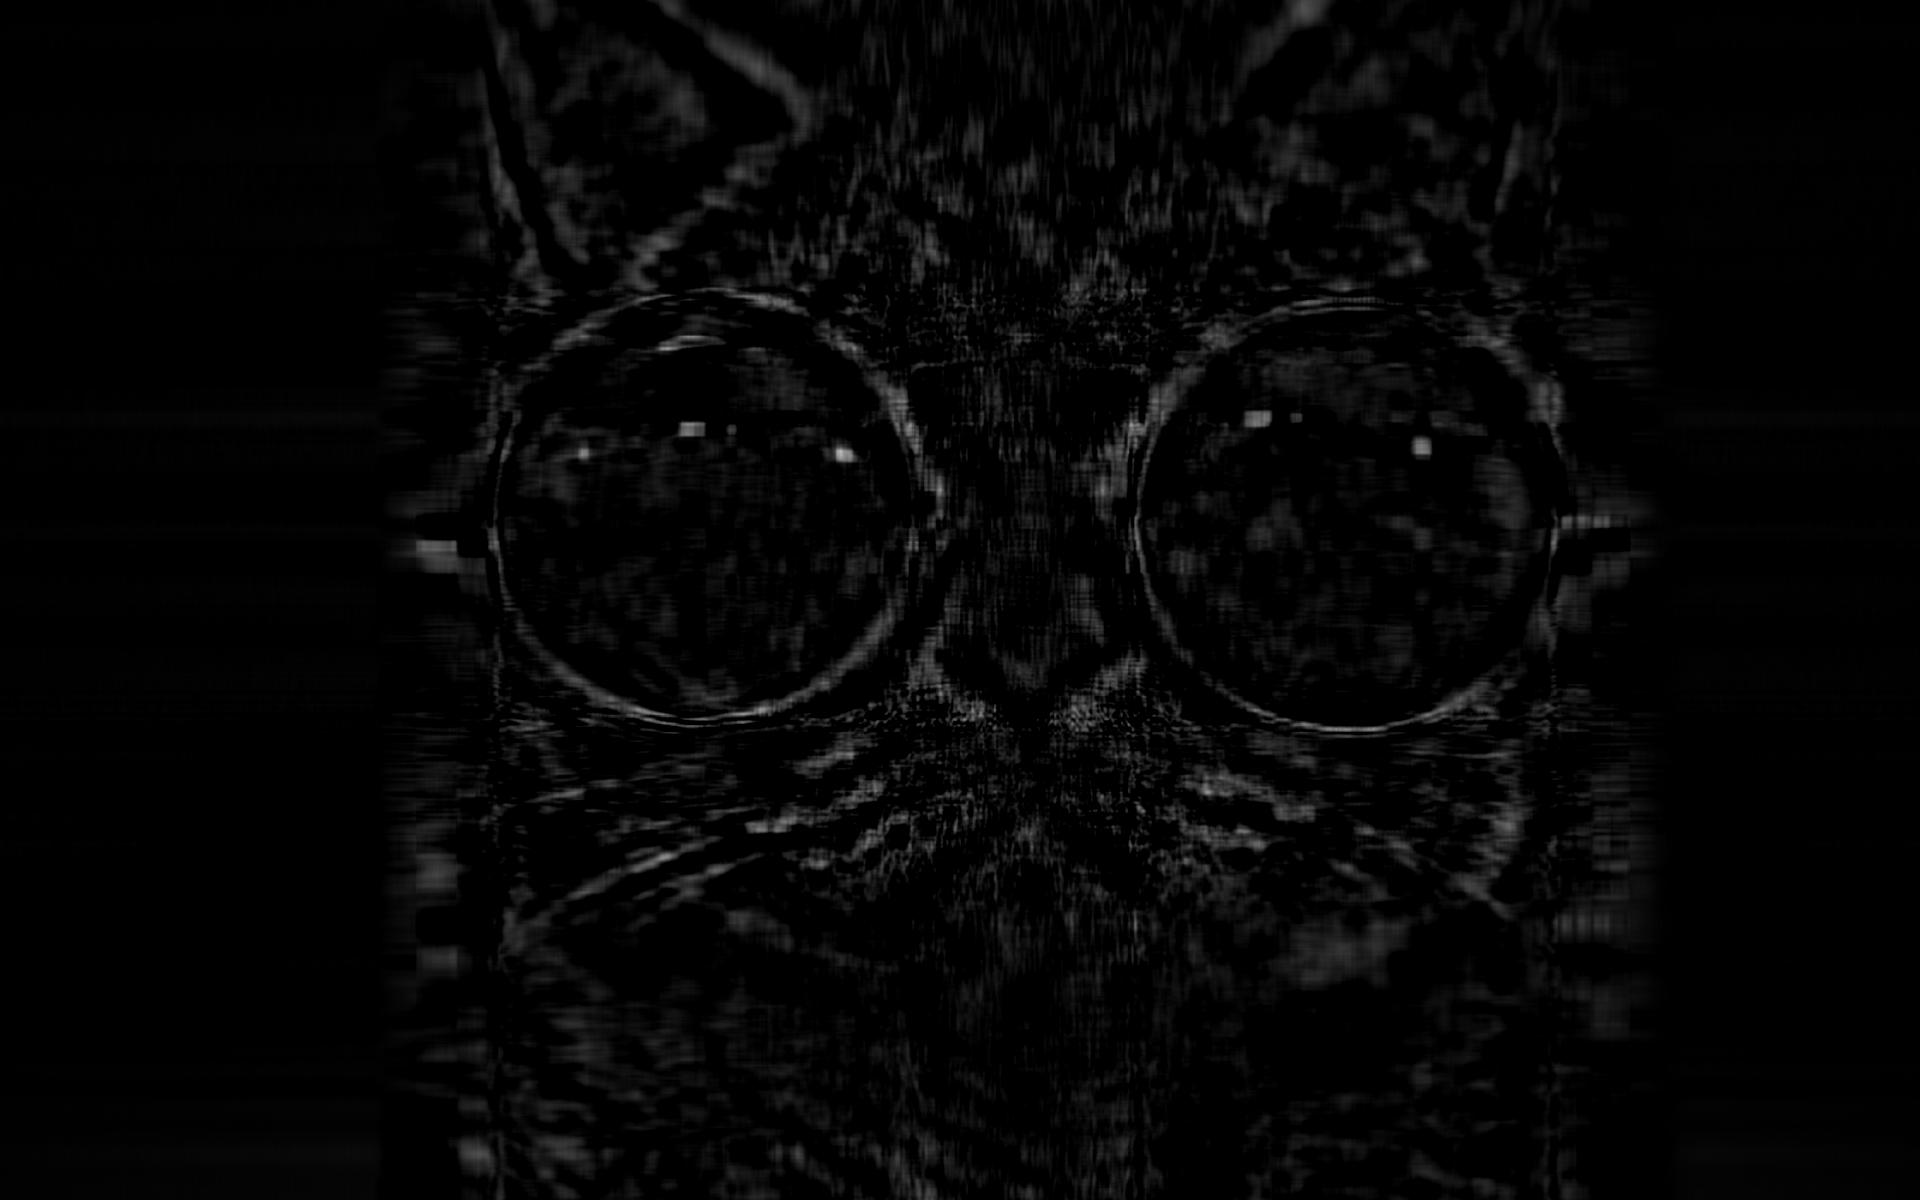
\includegraphics[width=.9\linewidth]{images/Cat10-30}
\subcaption{SW $\sigma_{10},\ldots,\sigma_{30}$.}
\end{subfigure}
\begin{subfigure}[c]{.3\textwidth}
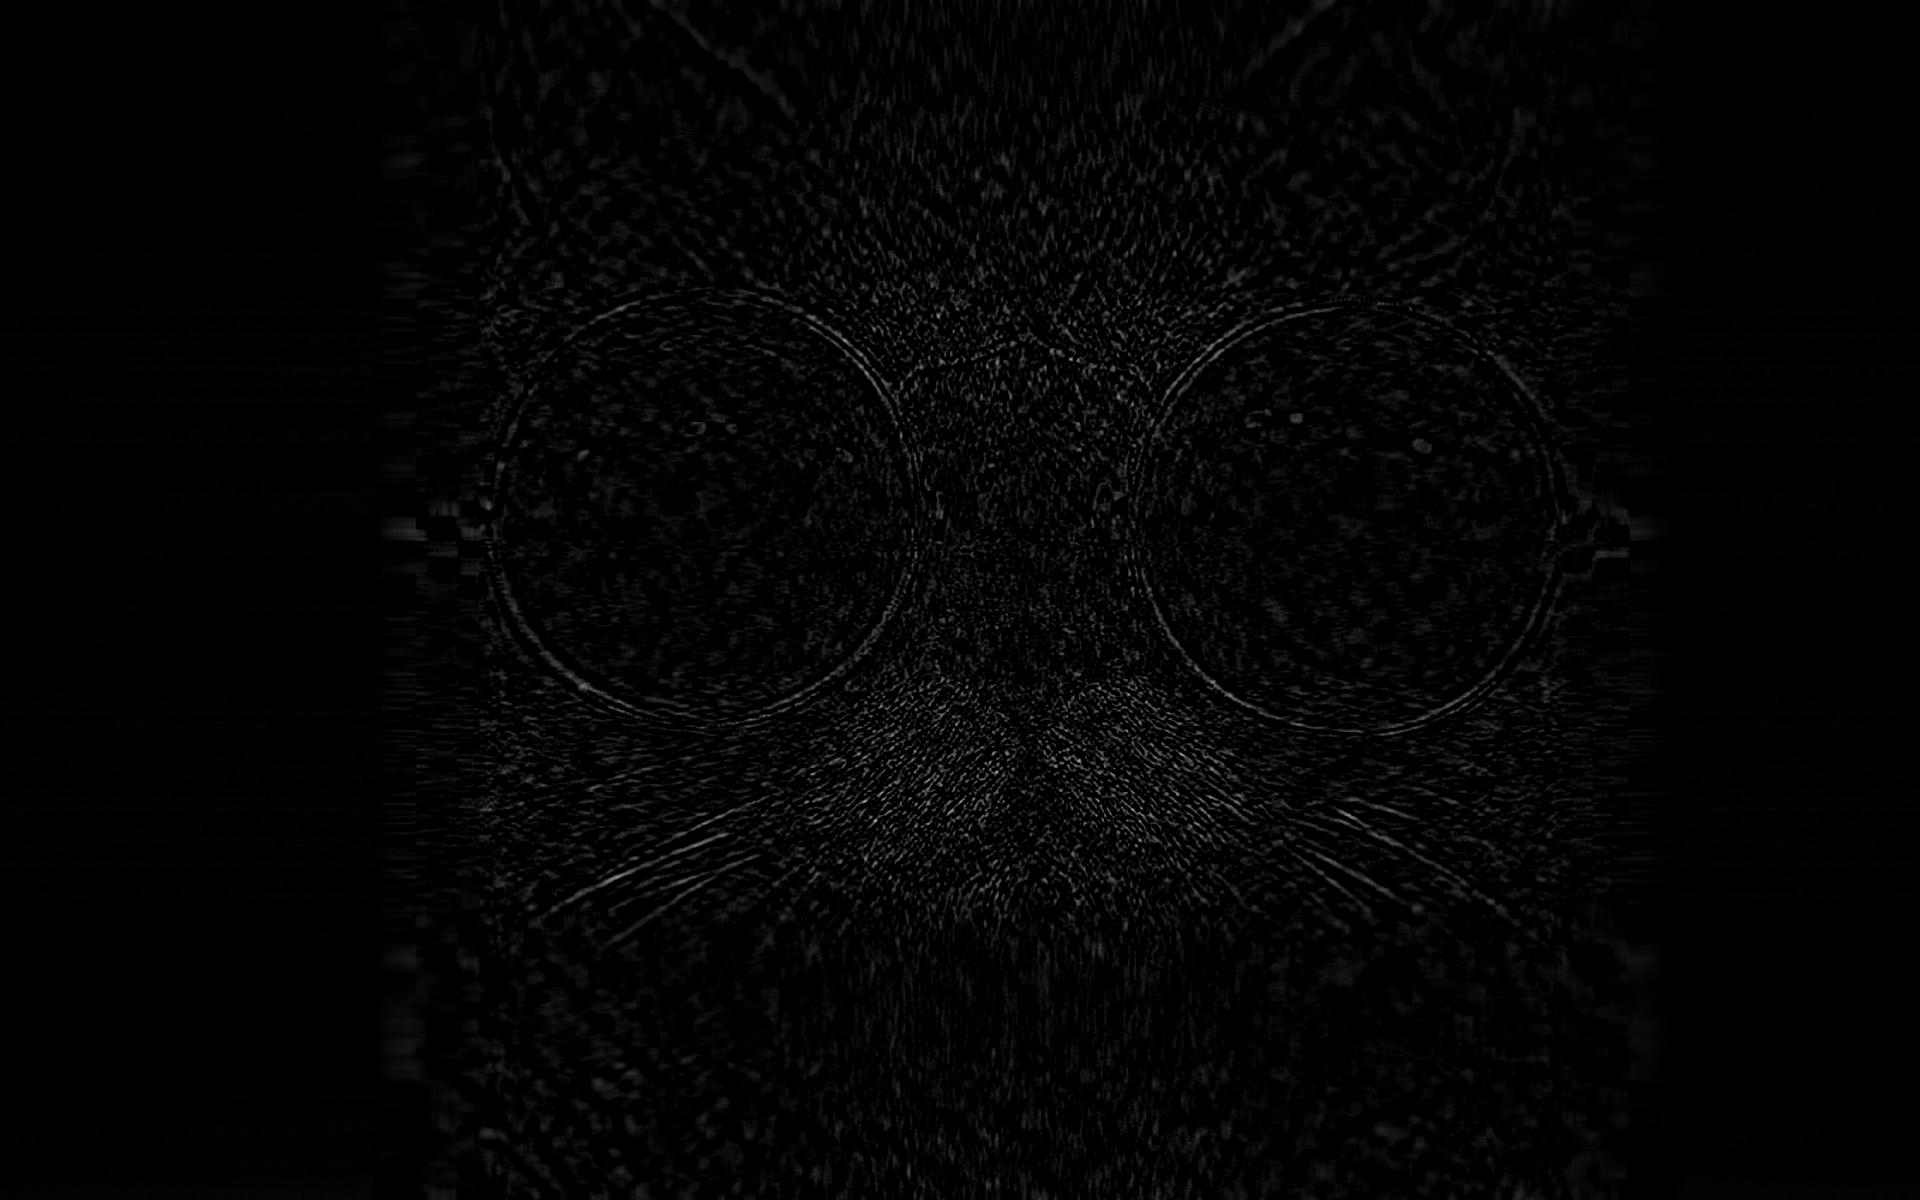
\includegraphics[width=.9\linewidth]{images/Cat40-90}
\subcaption{SW $\sigma_{40},\ldots,\sigma_{90}$.}
\end{subfigure}
\begin{subfigure}[c]{.3\textwidth}
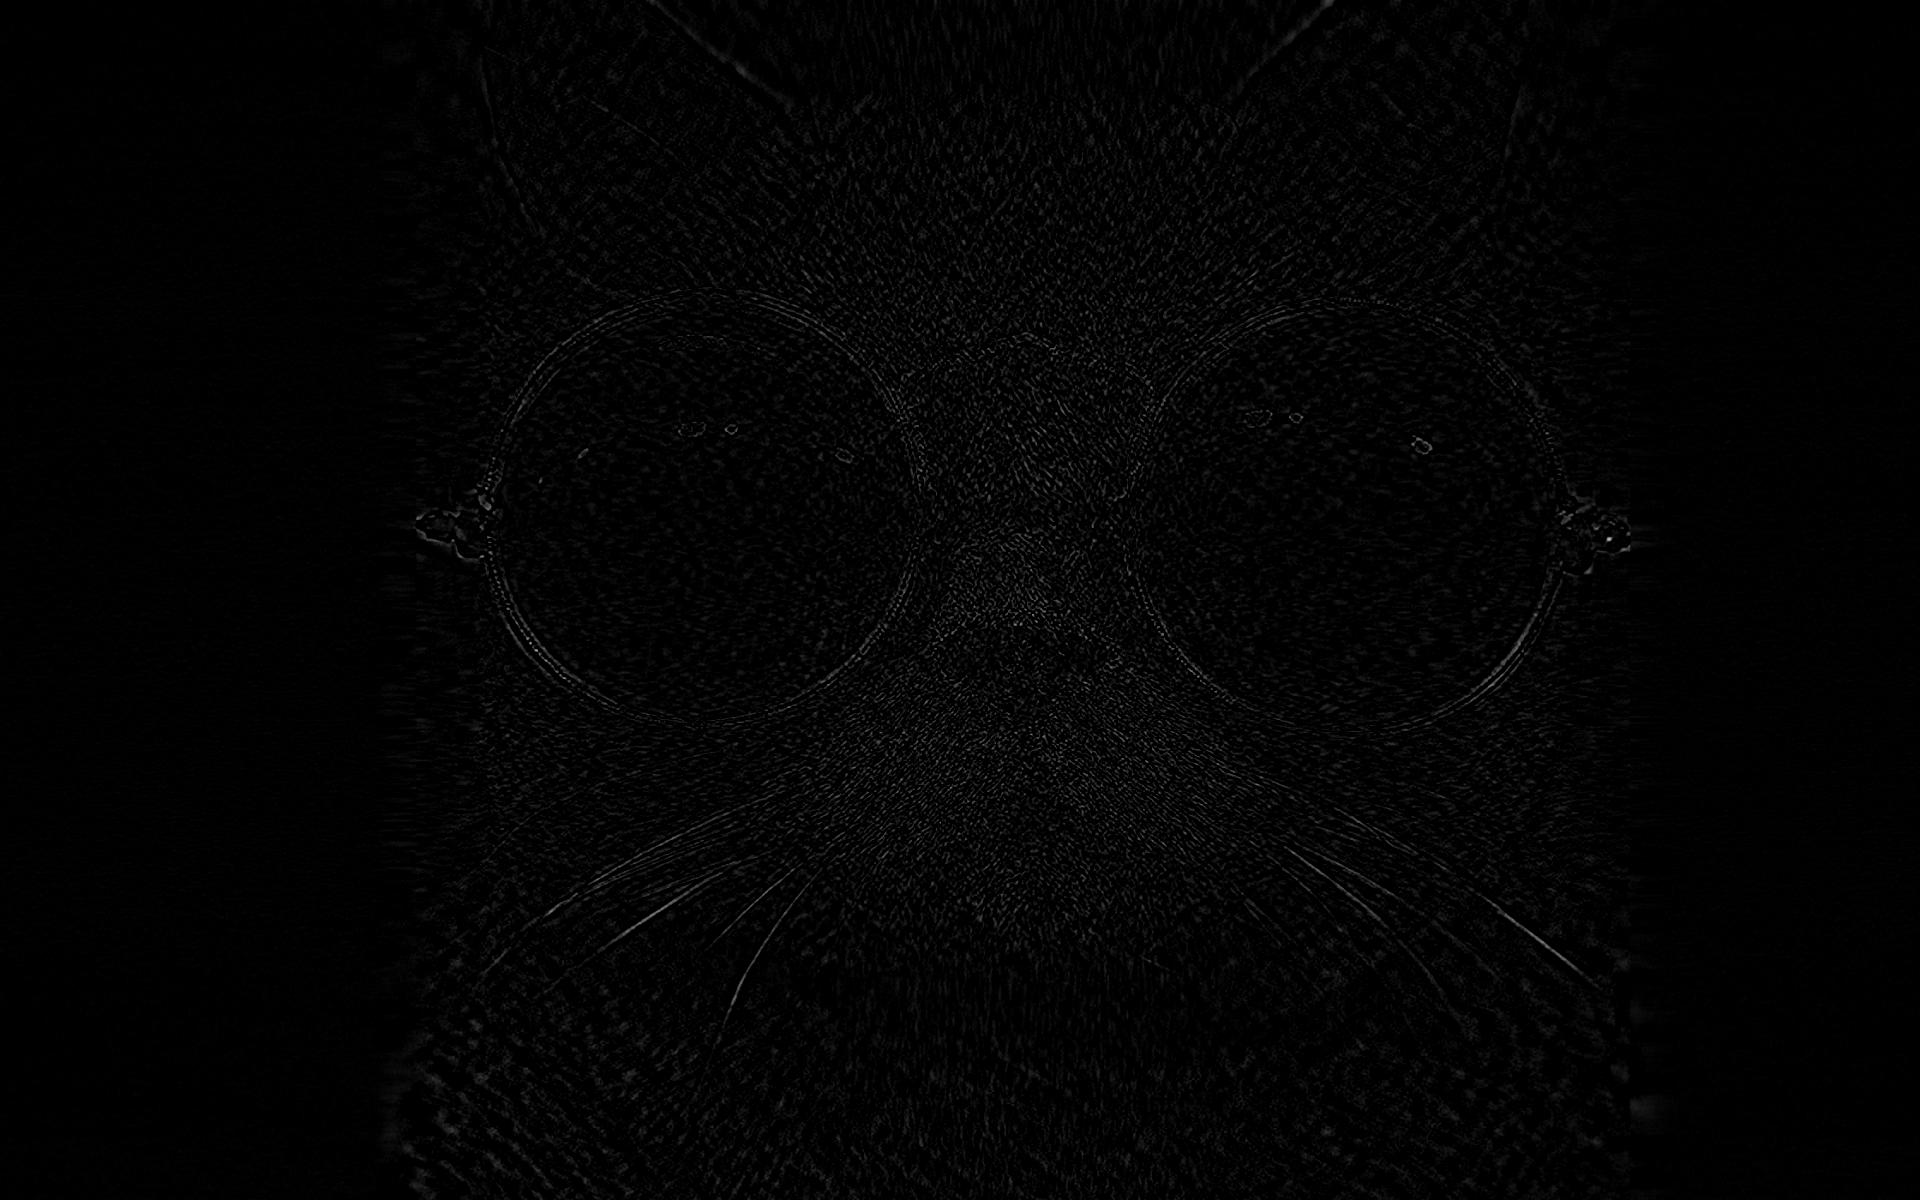
\includegraphics[width=.9\linewidth]{images/Cat100-400}
\subcaption{SW $\sigma_{100},\ldots,\sigma_{400}$.}
\end{subfigure}

\caption{Rekonstruktionsversuch von Abbildung \ref{chap1:im:cat}.}\label{chap1:im:catinterval}
\end{figure}

Die in Abbildung \ref{chap1:im:catinterval} gew"ahlte Filtrierung erscheint etwas ungl"ucklich, da das urspr"ungliche Bild kaum wieder zu erkennen ist.
Versuchen wir unser Gl"uck daher mit einer anderen Wahl von Singul"arwerten.

\newpage

\begin{figure}[h!]
\center
\begin{subfigure}[c]{.3\textwidth}
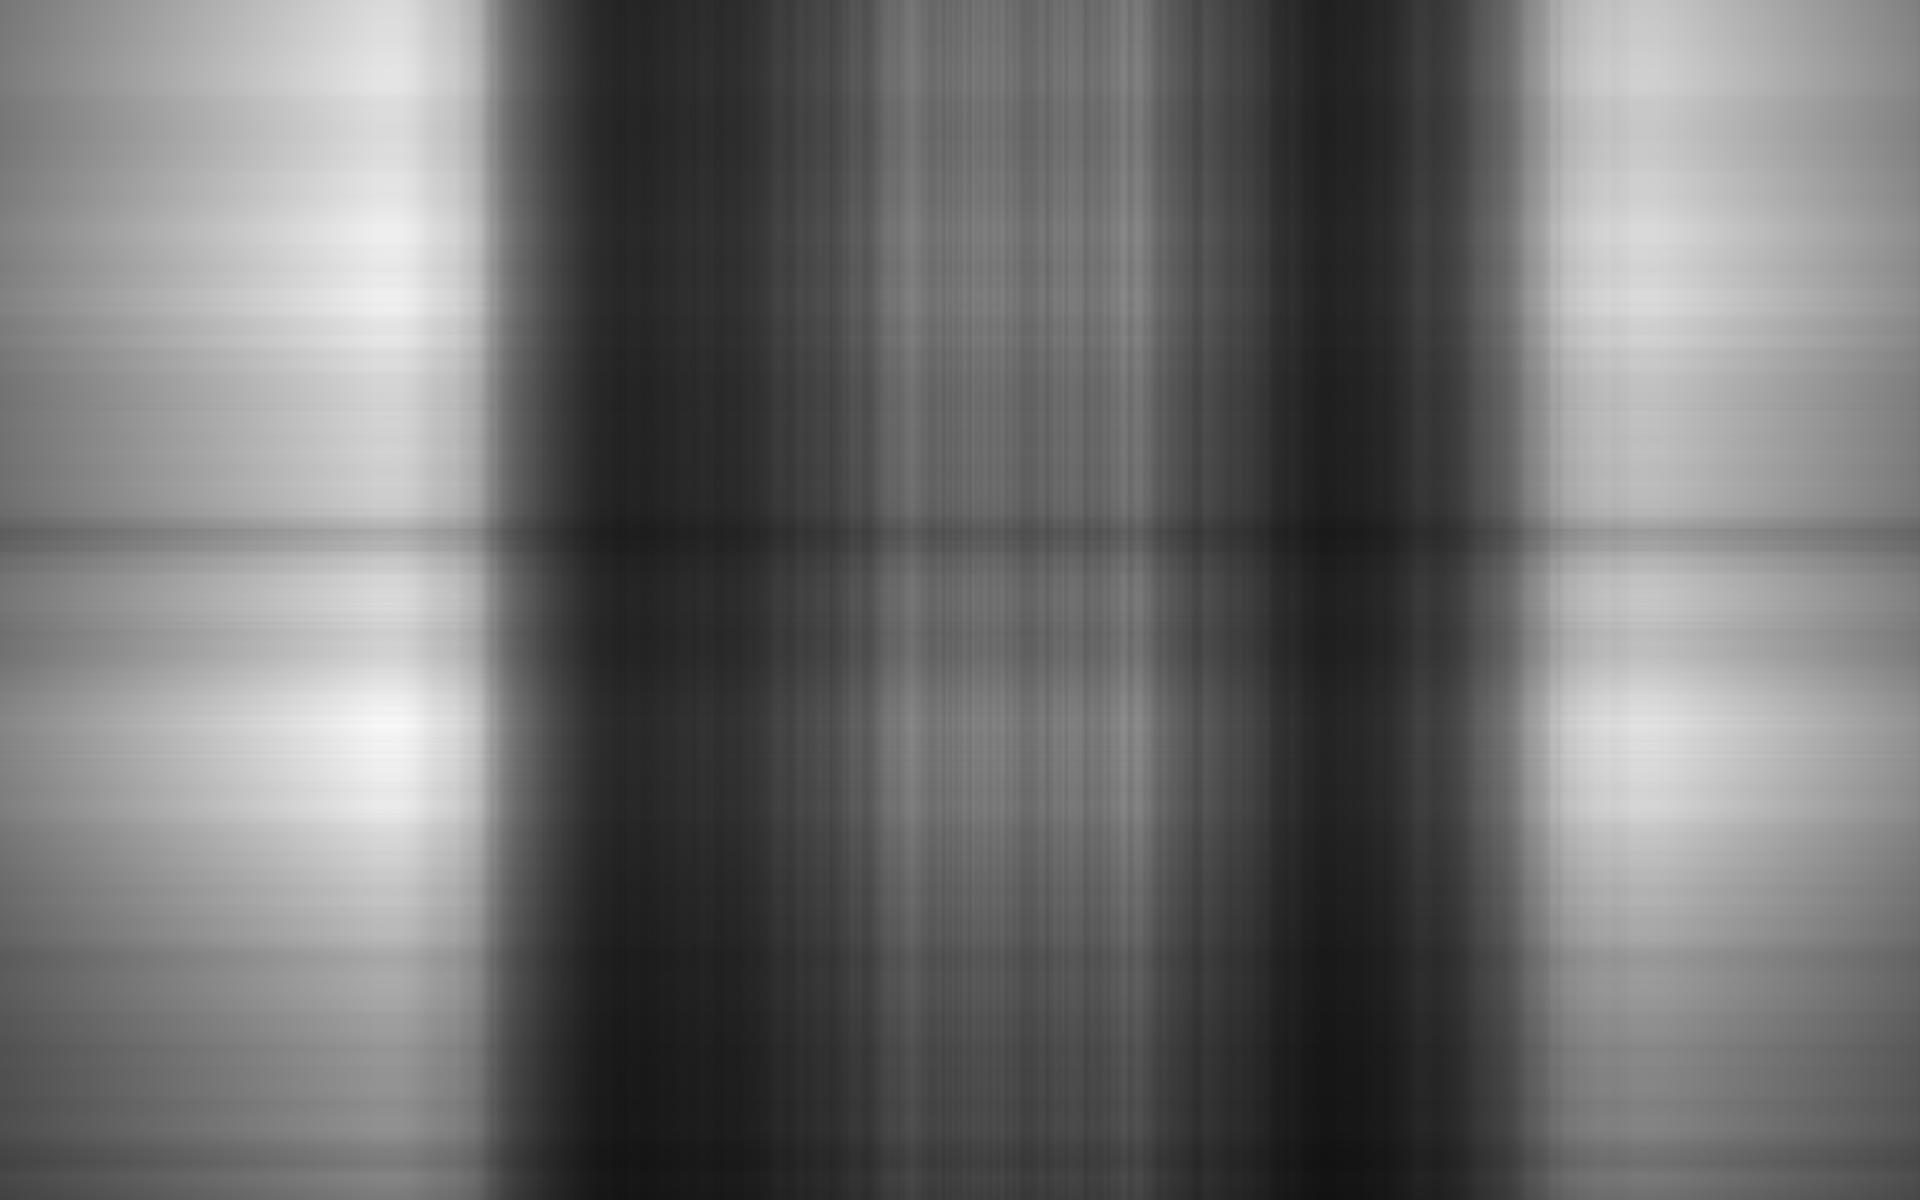
\includegraphics[width=.9\linewidth]{images/Cat1}
\subcaption{SW $\sigma_1$.}
\end{subfigure}
\begin{subfigure}[c]{.3\textwidth}
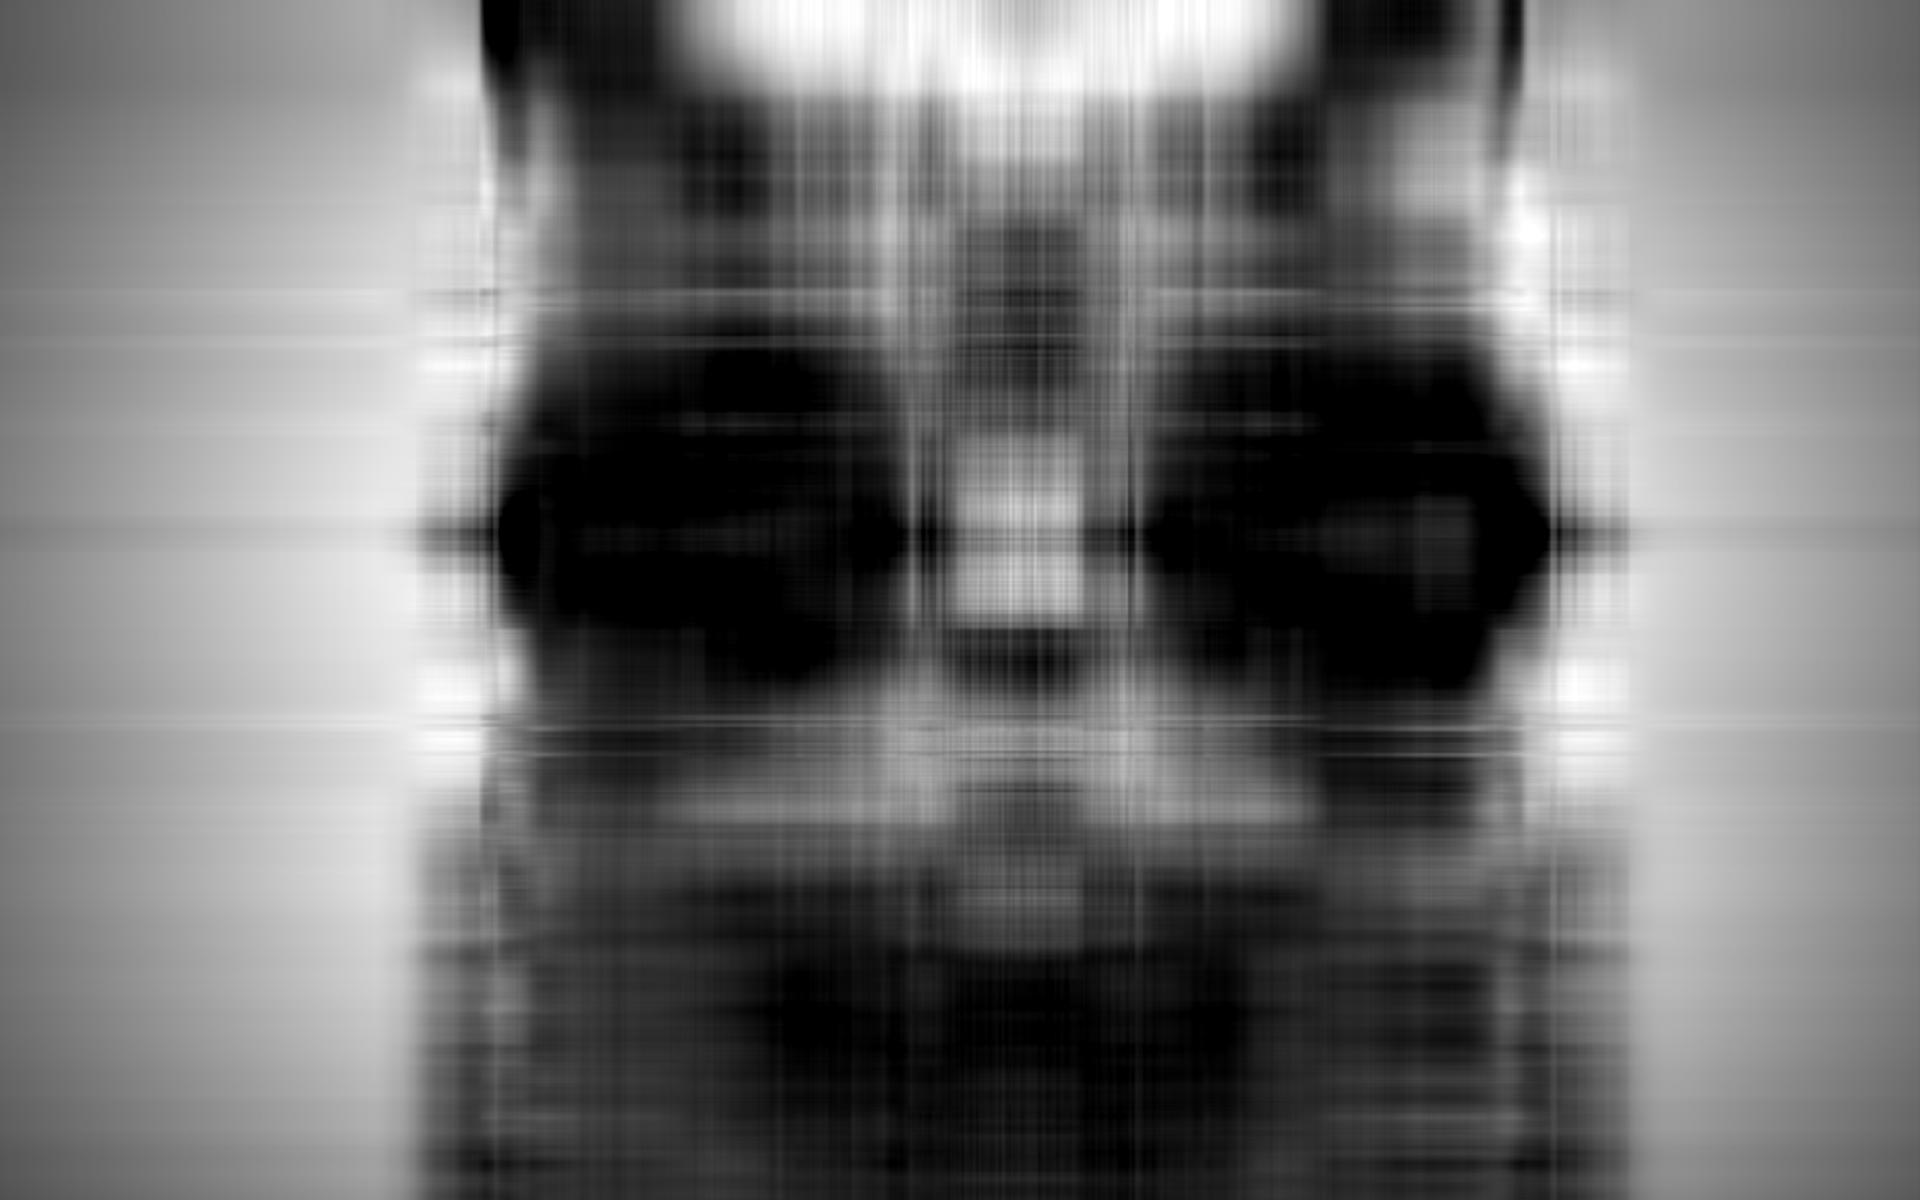
\includegraphics[width=.9\linewidth]{images/Cat5}
\subcaption{SW $\sigma_1,\ldots, \sigma_5$.}
\end{subfigure}
\begin{subfigure}[c]{.3\textwidth}
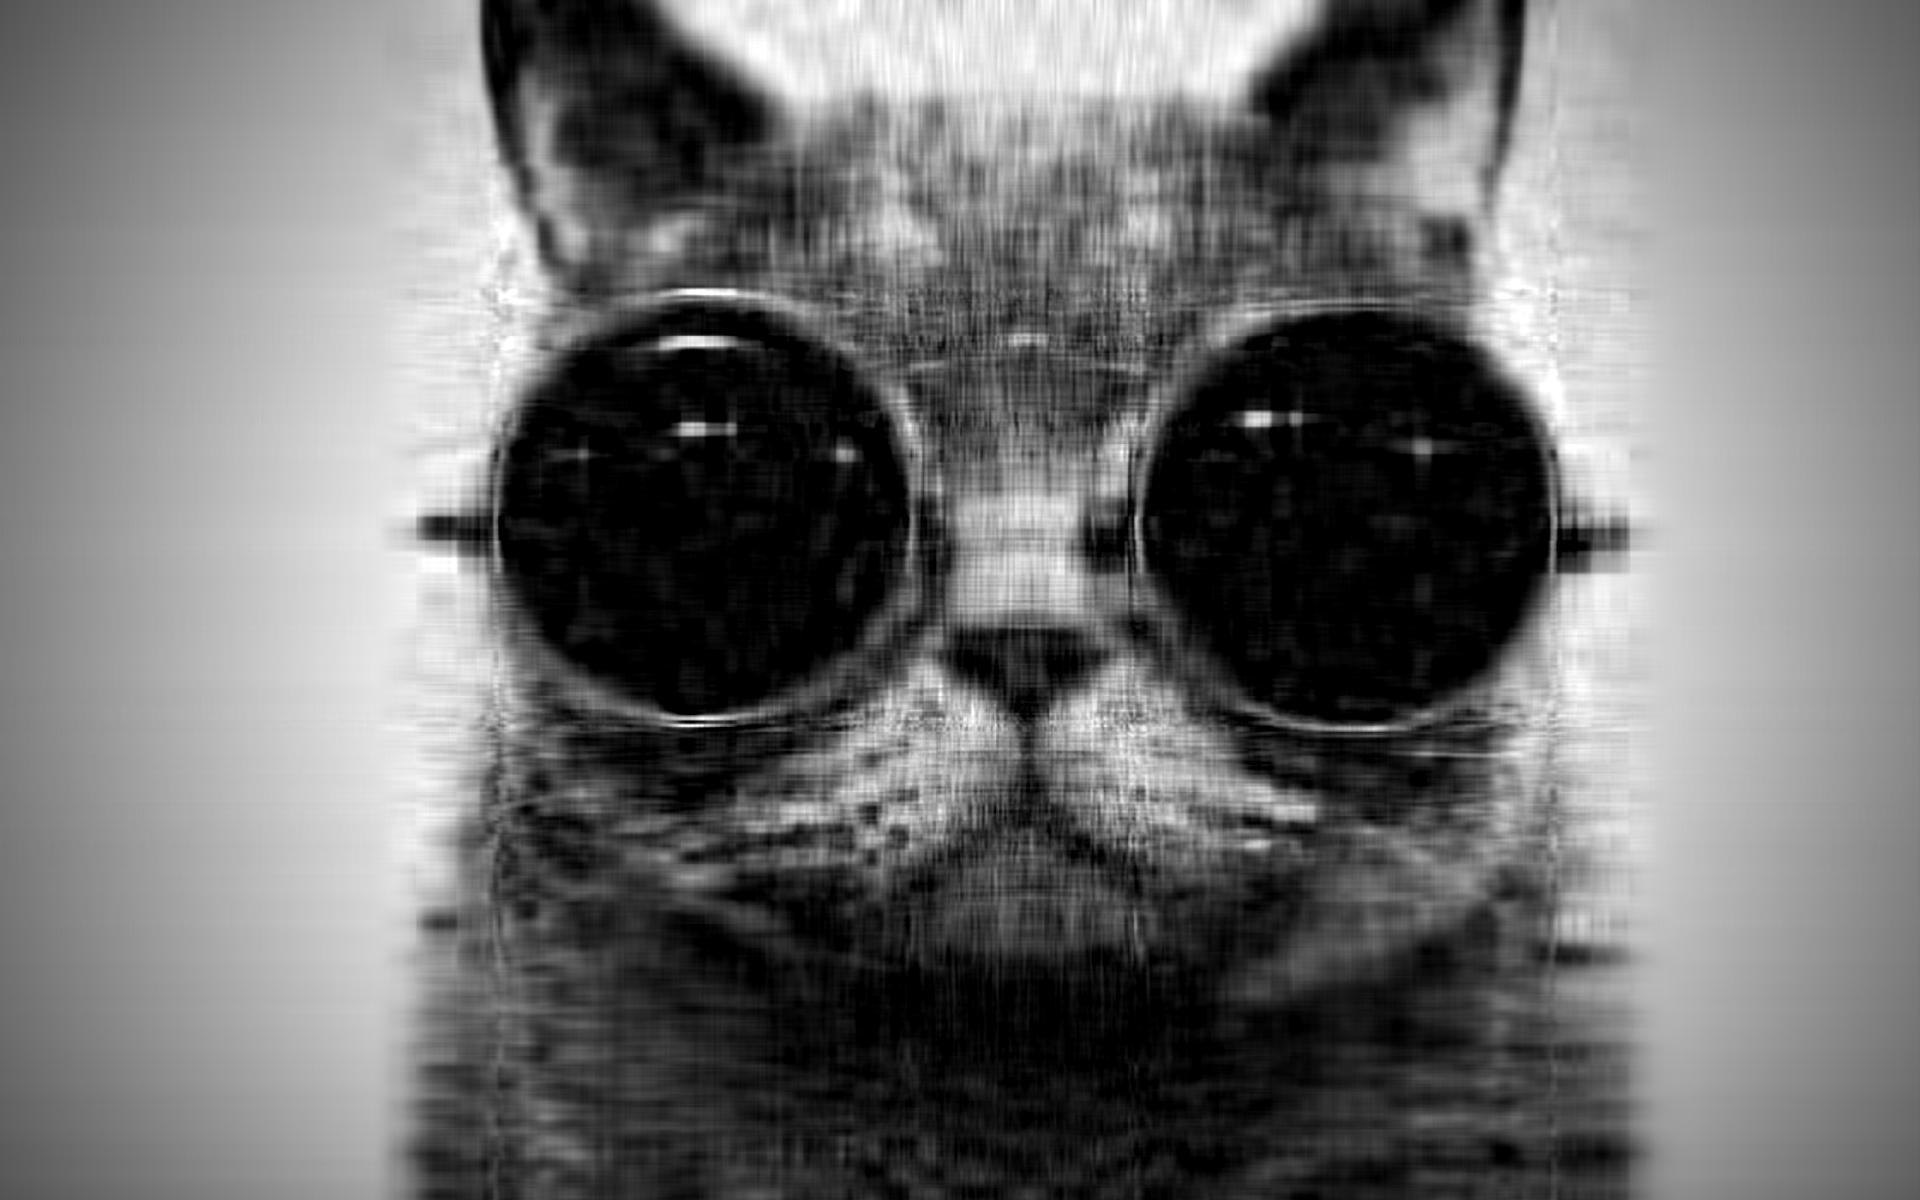
\includegraphics[width=.9\linewidth]{images/Cat20}
\subcaption{SW $\sigma_1,\ldots, \sigma_{20}$.}
\end{subfigure}

\vspace{0.4cm}
\begin{subfigure}[c]{.3\textwidth}
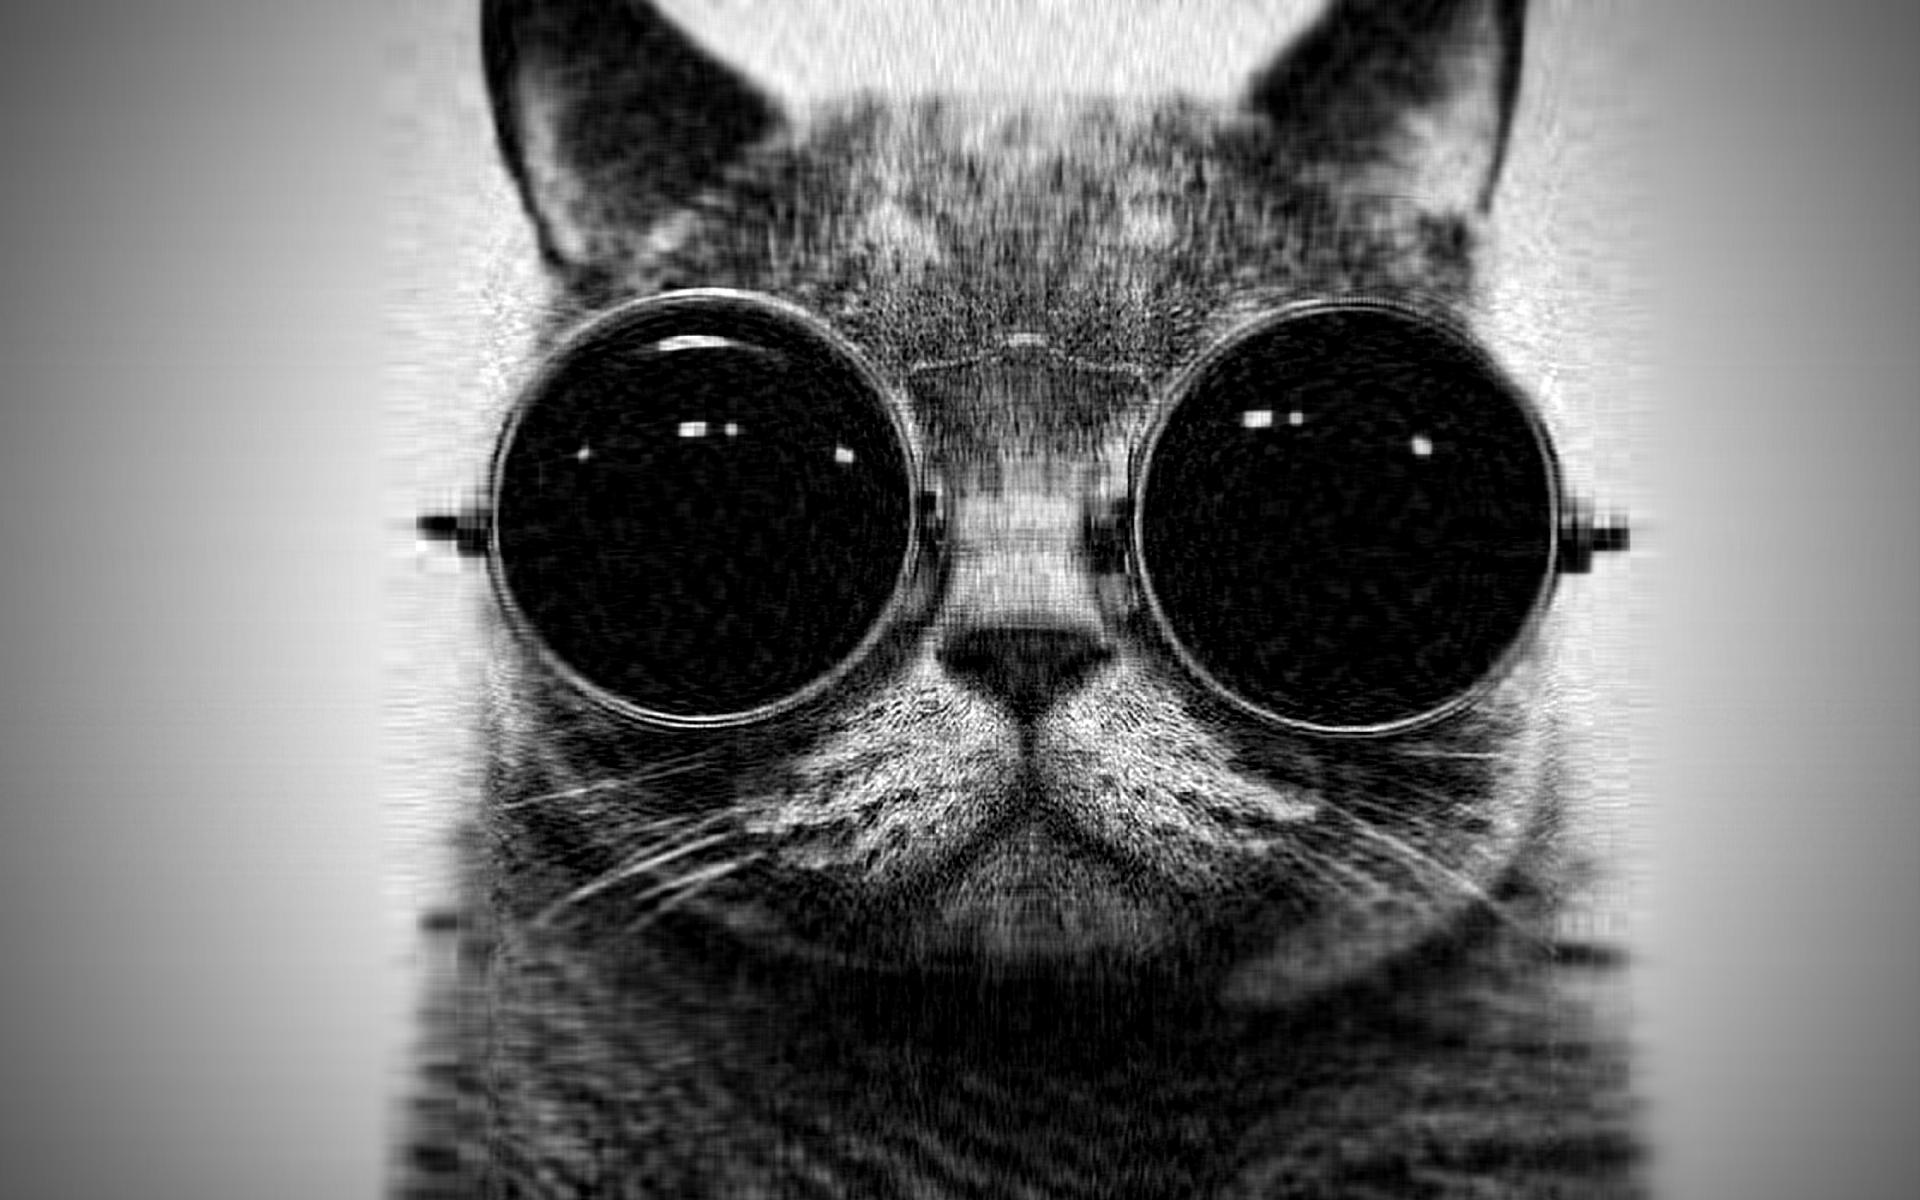
\includegraphics[width=.9\linewidth]{images/Cat50}
\subcaption{SW $\sigma_1,\ldots, \sigma_{50}$.}
\end{subfigure}
\begin{subfigure}[c]{.3\textwidth}
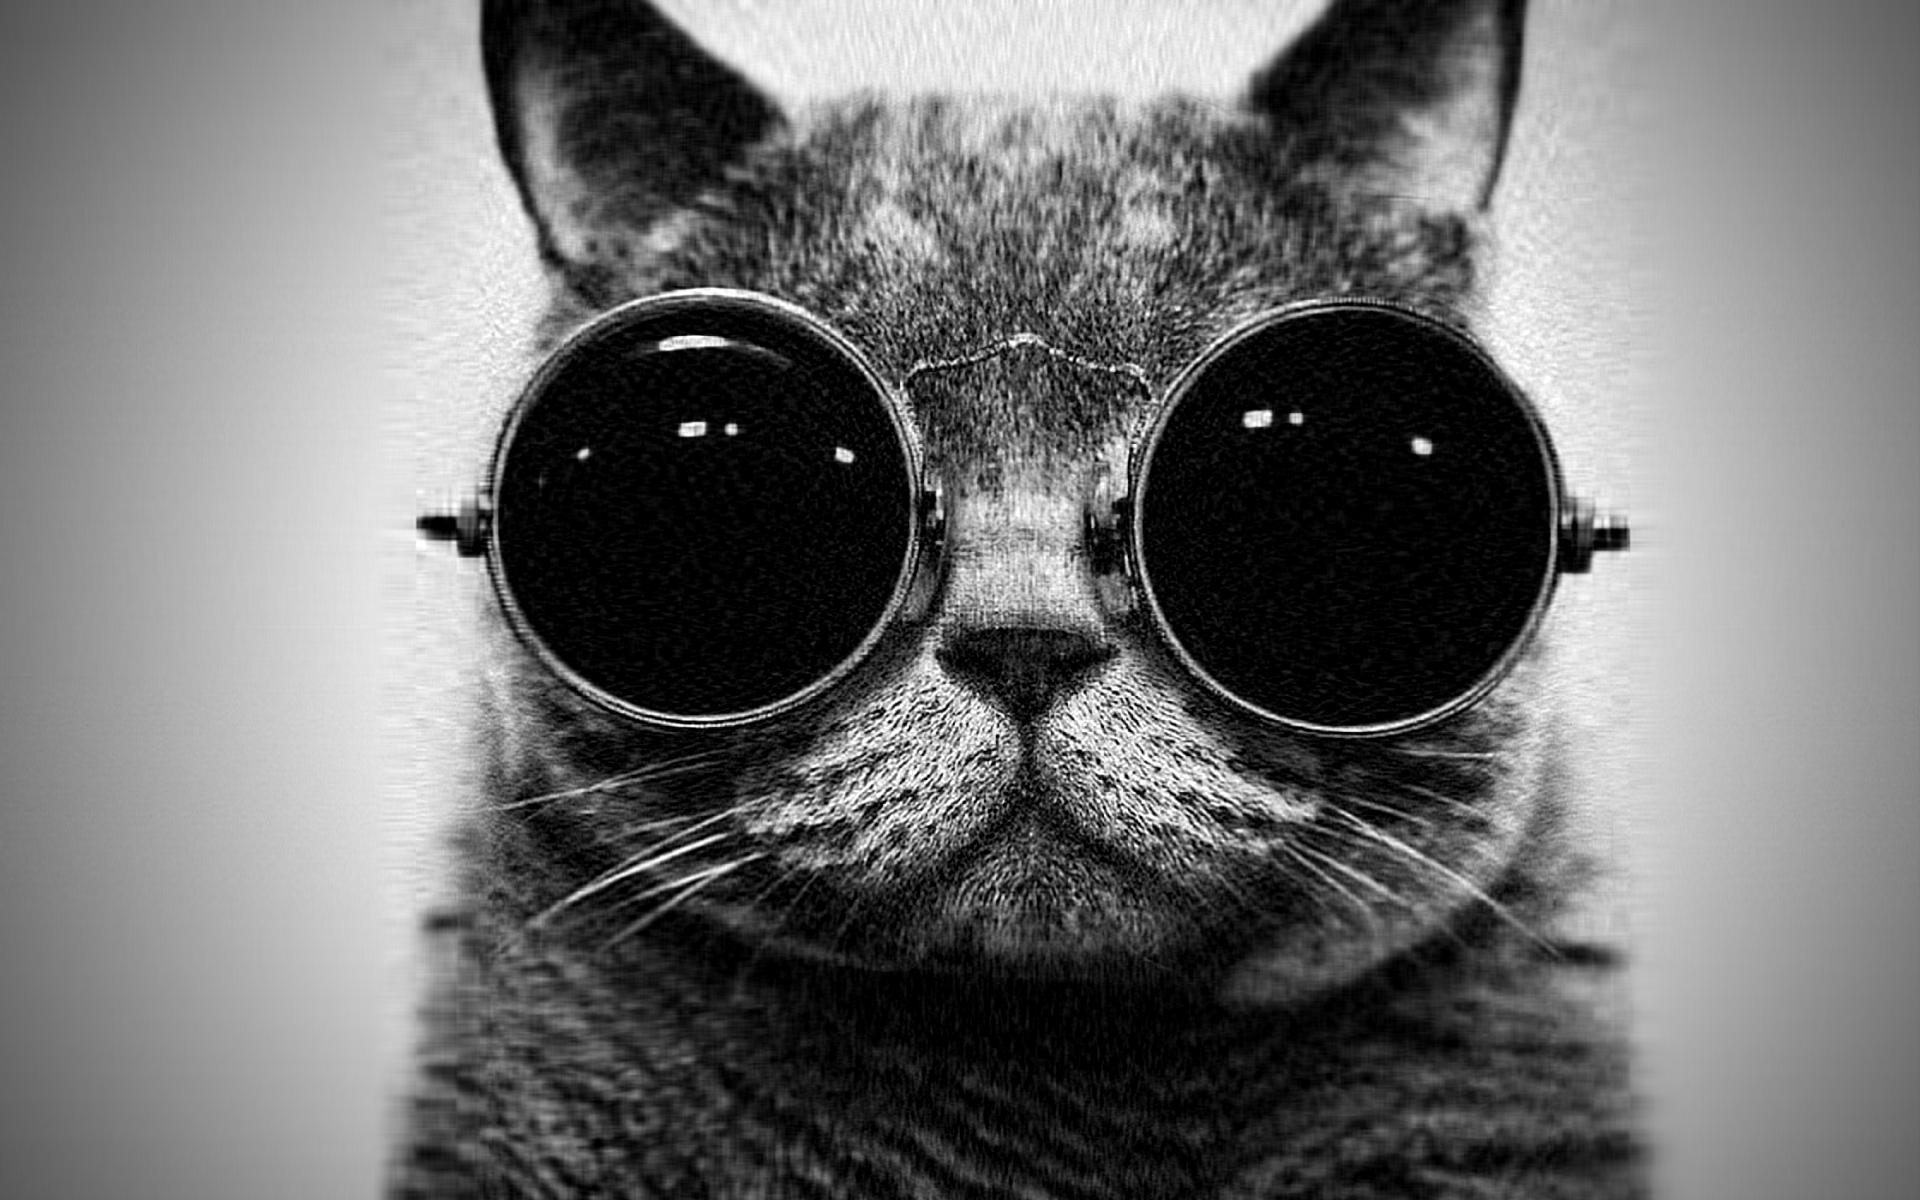
\includegraphics[width=.9\linewidth]{images/Cat100}
\subcaption{SW $\sigma_1,\ldots, \sigma_{100}$.}\label{im:chap1:subE}
\end{subfigure}
\begin{subfigure}[c]{.3\textwidth}
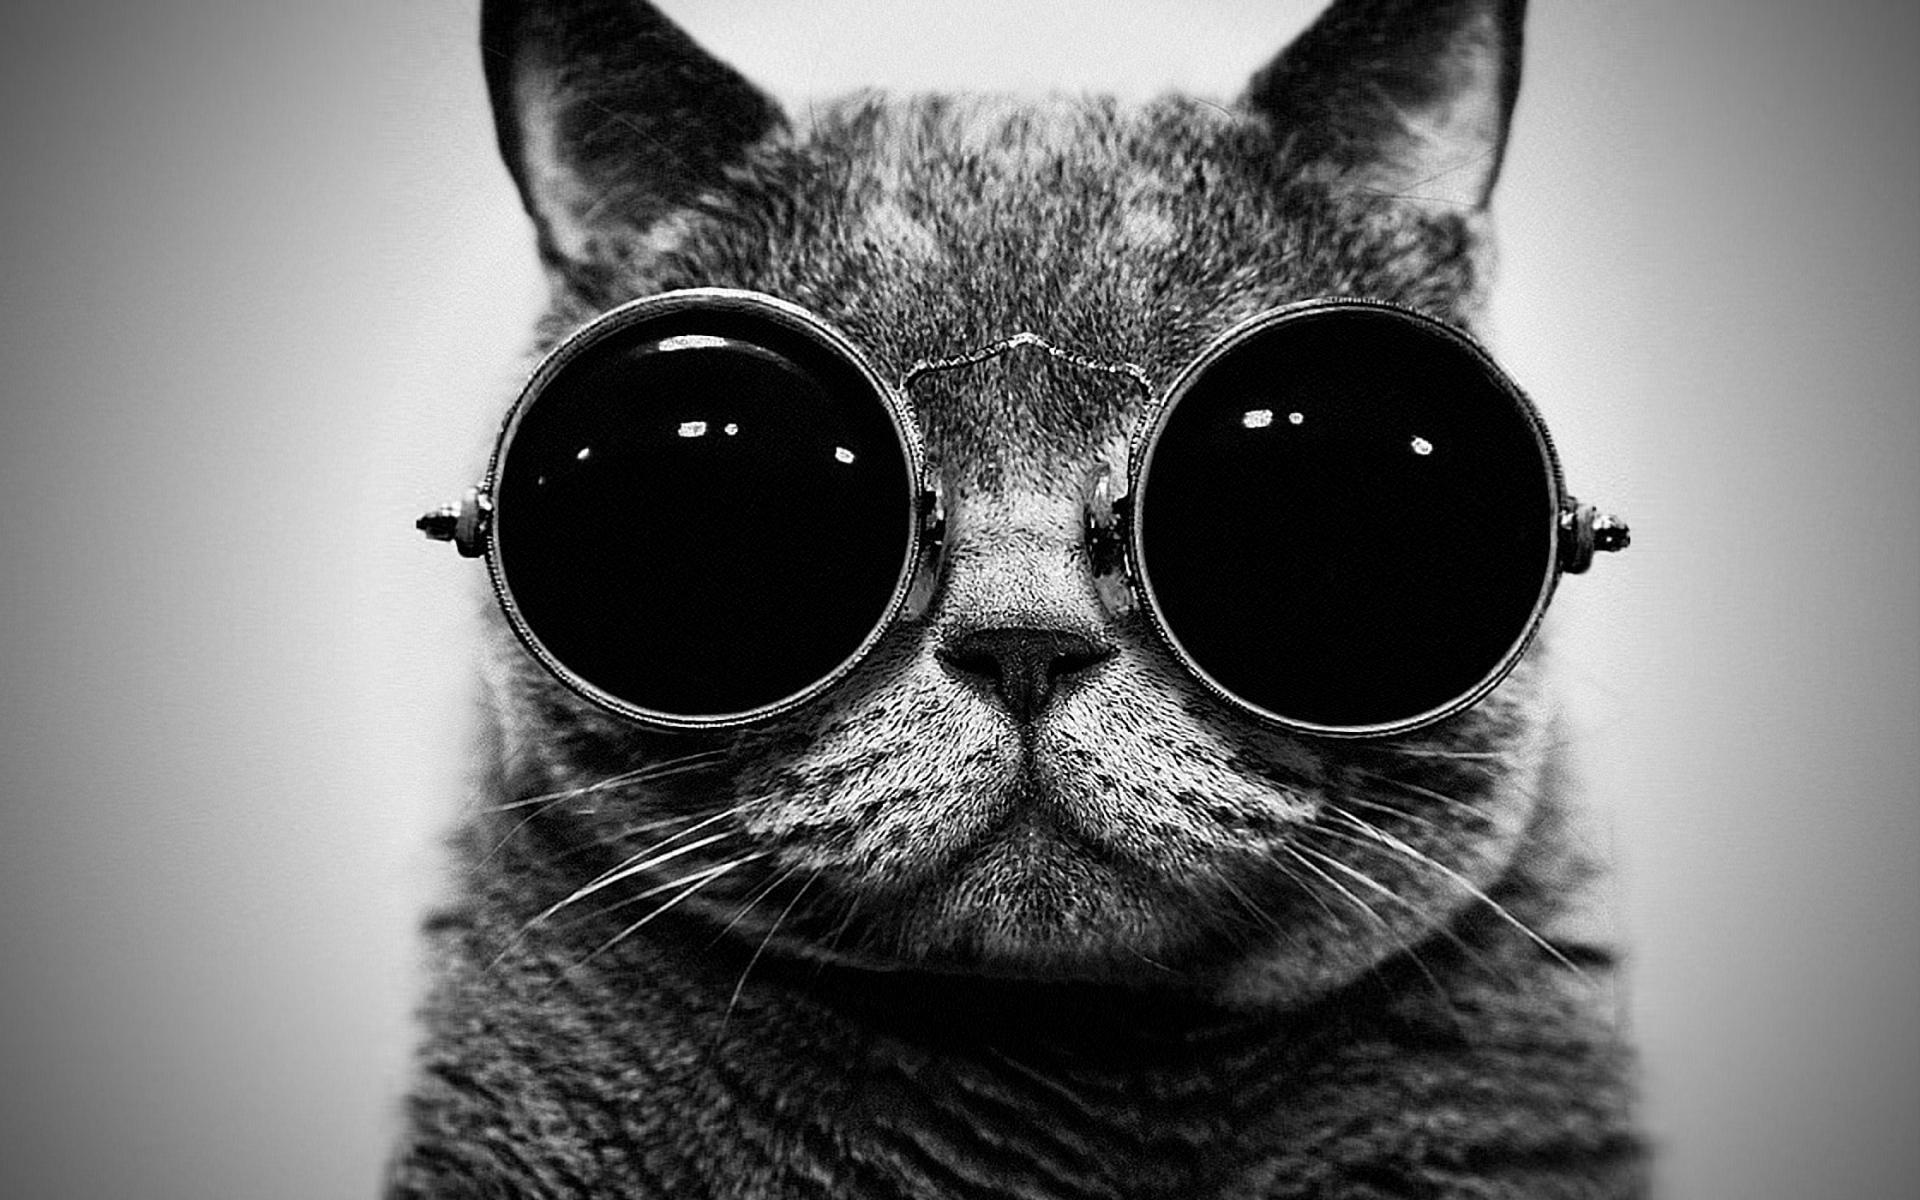
\includegraphics[width=.9\linewidth]{images/Cat300}
\subcaption{SW $\sigma_1,\ldots, \sigma_{300}$.}\label{im:chap1:subF}
\end{subfigure}

\caption{Approximation von Abbildung \ref{chap1:im:cat} mittels Singul"arwertzerlegung.}
\end{figure}

Dieser Versuch wirkt "uberzeugender. Bereits bei Figur \ref{im:chap1:subE} ist ein genauer Blick erforderlich, um die Makel der Komprimierung zu erkennen.
Bei der Verwendung der ersten 300 SW ist es nahezu unm"oglich einen Unterschied zum Original festzustellen.
Es ist also zu "uberlegen, ob man sich mit der Qualit"at der Figur \ref{im:chap1:subF} zufrieden geben m"ochte und statt Abbildung \ref{chap1:im:cat} nicht einfach dieses abspeichert.\\

Nun ist das Approximieren von Bildern ein sehr spezieller Fall des Filterns von Eigenwerten und die Berechnung der Singul"arwertzerlegung nicht immer zweckm"a"sig oder m"oglich.
Daher setzt sich diese Arbeit mit Alternativen auseinander, die dem Filtern dienlich sind. Dabei werden neben den mathematischen Ideen dieser Alternativen auch M"oglichkeiten der Implementation vorgestellt.\\

Im dritten Kapitel werden zun"achst zwei Methoden pr"asentiert, die als Werkzeuge zum Filtern von Eigenpaaren dienlich sind.
Daran wird sich nach einer kurzen analytischen Illustration dieser Verfahren eine Diskussion anschlie"sen, bei der untersucht wird, wie es um die praktische Umsetzbarkeit der Verfahren bestellt ist.
Wir werden feststellen, dass sich die Algorithmen kombinieren und modifizieren lassen und zu einem Verfahren f"uhren, welches in der Literatur als FEAST-Algorithmus gehandelt wird. Zum Abschluss begeben wir uns in das \glqq Numerik-Labor\grqq\ und werden die Grenzen der Algorithmen austesten.\\

Bevor es konkreter wird, erinnert der folgende Abschnitt an einige mathematische Grundlagen, die als helfende Handreichung das Lesen dieser Schrift mehr zur Freude, denn zur Schikane machen soll.
